\section{TP 10}
%\addcontentsline{toc}{section}{TP 10}


\subsection*{Exercice 1}
Soit $G = (P, F)$ un graphe d'affiliations ($P$ rep\'{e}sente les personnes et $F$ les focus). On d\'{e}finit le \emph{graphe projet\'{e} sur les personnes} comme \'{e}tant un graphe avec ensemble de sommets $P$ et tel qu'il existe un lien entre deux personnes s'il existe un focus commun aux deux personnes dans $G$. \\

On consid\`{e}re le graphe d'affiliations suivant.
\begin{center}
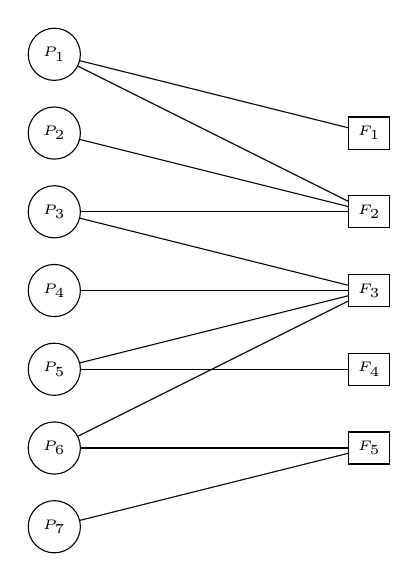
\begin{tikzpicture}
\node[draw, circle] at (0, 0) (P1) {\tiny $P_1$};
\node[draw, circle] at (0, -1) (P2) {\tiny $P_2$};
\node[draw, circle] at (0, -2) (P3) {\tiny $P_3$};
\node[draw, circle] at (0, -3) (P4) {\tiny $P_4$};
\node[draw, circle] at (0, -4) (P5) {\tiny $P_5$};
\node[draw, circle] at (0, -5) (P6) {\tiny $P_6$};
\node[draw, circle] at (0, -6) (P7) {\tiny $P_7$};
\node[draw, rectangle] at (4, -1) (F1) {\tiny $F_1$};
\node[draw, rectangle] at (4, -2) (F2) {\tiny $F_2$};
\node[draw, rectangle] at (4, -3) (F3) {\tiny $F_3$};
\node[draw, rectangle] at (4, -4) (F4) {\tiny $F_4$};
\node[draw, rectangle] at (4, -5) (F5) {\tiny $F_5$};
\draw (P1) -- (F1);
\draw (P1) -- (F2);
\draw (P2) -- (F2);
\draw (P3) -- (F2);
\draw (P3) -- (F3);
\draw (P4) -- (F3);
\draw (P5) -- (F3);
\draw (P5) -- (F4);
\draw (P6) -- (F3);
\draw (P6) -- (F5);
\draw (P7) -- (F5);
\end{tikzpicture}
\end{center}

\begin{enumerate}
\item Calculez le graphe projet\'{e} sur les personnes.

\item Donnez, si possible, un autre graphe d'affiliations avec la m\^{e}me projection sur les personnes.
\end{enumerate}

    \subsubsection*{Solution}
    La projection sur les personnes donne le graphe suivant :

    \begin{center}
    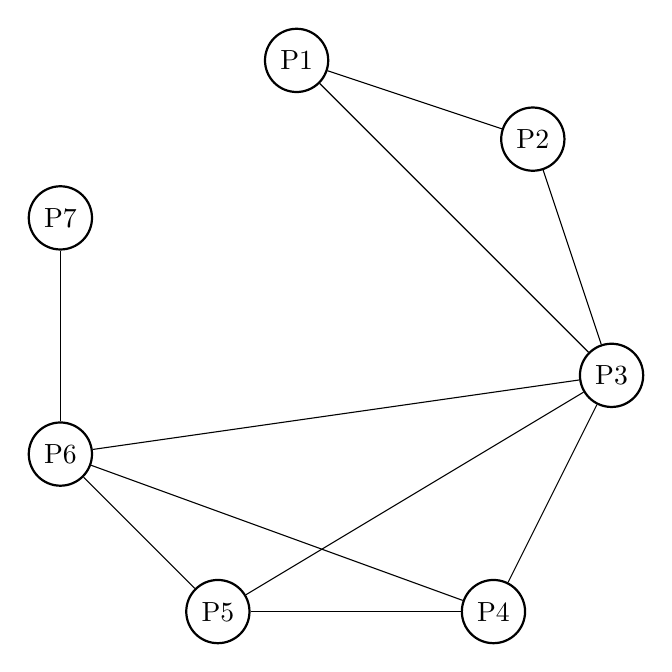
\begin{tikzpicture}
    \tikzstyle{node}=[circle,draw,thick,fill=white]
    \node[node] (P1) at (0,0) {P1};
    \node[node] (P2) at (3,-1) {P2};
    \node[node] (P3) at (4,-4) {P3};
    \node[node] (P4) at (2.5,-7) {P4};
    \node[node] (P5) at (-1,-7) {P5};
    \node[node] (P6) at (-3,-5) {P6};
    \node[node] (P7) at (-3,-2) {P7};
    \draw (P1) -- (P2);
    \draw (P1) -- (P3);
    \draw (P2) -- (P3);
    \draw (P3) -- (P4);
    \draw (P3) -- (P5);
    \draw (P3) -- (P6);
    \draw (P4) -- (P5);
    \draw (P4) -- (P6);
    \draw (P5) -- (P6);
    \draw (P6) -- (P7);
    \end{tikzpicture}
    \end{center}

    Il est facile d'obtenir la même projection avec un graphe d'affiliations différent.
    On peut pour cela rajouter un (ou plusieurs) focus relié(s) à une seule personne.
    Il est aussi possible de diviser un focus en 3 focus (vu plus en détail à la question 3).


\subsection*{Exercice 2}
\begin{enumerate}
\item
Calculez de graphe projet\'{e} sur les personnes du graphe d'affiliations suivant.
\begin{center}
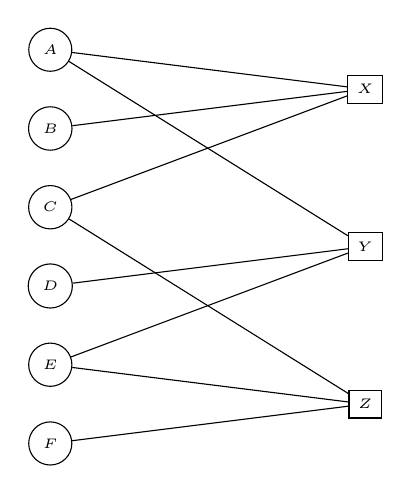
\begin{tikzpicture}
\node[draw, circle] at (0, 0) (A) {\tiny $A$};
\node[draw, circle] at (0, -1) (B) {\tiny $B$};
\node[draw, circle] at (0, -2) (C) {\tiny $C$};
\node[draw, circle] at (0, -3) (D) {\tiny $D$};
\node[draw, circle] at (0, -4) (E) {\tiny $E$};
\node[draw, circle] at (0, -5) (F) {\tiny $F$};
\node[draw, rectangle] at (4, -0.5) (X) {\tiny $X$};
\node[draw, rectangle] at (4, -2.5) (Y) {\tiny $Y$};
\node[draw, rectangle] at (4, -4.5) (Z) {\tiny $Z$};
\draw (A) -- (X);
\draw (A) -- (Y);
\draw (B) -- (X);
\draw (C) -- (X);
\draw (C) -- (Z);
\draw (D) -- (Y);
\draw (E) -- (Y);
\draw (E) -- (Z);
\draw (F) -- (Z);
\end{tikzpicture}
\end{center}
\item Dans le graphe r\'{e}sultant de la projection, expliquez la diff\`{e}rence qualitative entre le triangle $A$-$E$-$C$ et les autes.
\end{enumerate}

    \subsubsection*{Solution}
    Le graphe projeté sur les personnes est le suivant :

    \begin{center}
    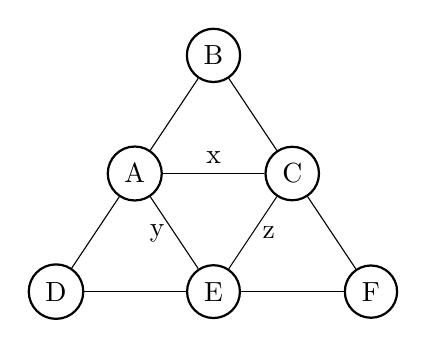
\begin{tikzpicture}
    \tikzstyle{node}=[circle,draw,thick,fill=white]
    \node[node] (A) at (1,1.5) {A};
    \node[node] (B) at (2,3) {B};
    \node[node] (C) at (3,1.5) {C};
    \node[node] (D) at (0,0) {D};
    \node[node] (E) at (2,0) {E};
    \node[node] (F) at (4,0) {F};
    \draw (A) -- (B);
    \draw (A) -- (C) node[midway,above]{x};
    \draw (A) -- (D);
    \draw (A) -- (E) node[midway,left]{y};
    \draw (B) -- (C);
    \draw (C) -- (E) node[midway,right]{z};
    \draw (C) -- (F);
    \draw (D) -- (E);
    \draw (E) -- (F);
    \end{tikzpicture}
    \end{center}

    La différence entre le triangle A-E-C et les autres est que celui-ci ne correspond pas à 1 seul et unique focus.
    En effet, A-C correspond à x, A-E à y, et C-E à z.\\
    Il y a d'ailleurs un théorème important qui signale que lorsque la projection sur les personnes contient un sous-graphe complet, cela n'implique pas l'existence d'un focus commun à tous ses noeuds.


\subsection*{Exercice 3}
Quel est le nombre minimum de focus qu'il faut avoir dans un graphe d'affiliation
pour que sa projection sur les personnes soit le graphe complet si il n'y a pas de focus commum \`{a} toutes les personnes?

    \subsubsection*{Solution}
    Il faut au minimum \textbf{trois} focus pour que la projection sur les personnes donne un graphe complet sans avoir de focus commun à tous.

    On prouve tout d'abord que cela ne fonctionne pas avec moins de 3 focus.\\
    Si l'on prend 1 seul focus, le seul moyen d'obtenir le graphe complet est de relier toutes les personnes à ce focus, et on aura donc 1 focus commun à tous.\\
    Si l'on prend 2 focus, on peut démarrer avec 3 personnes et voir qu'il est impossible d'obtenir $K_3$ avec la projection sur les personnes.
    En effet, pour éviter d'avoir un focus commun, on prend 2 de ces personnes et on les relie chacune à un focus différent.
    La $3^{\text{ème}}$ personne est reliée aux 2 focus, et donc aux 2 autres.
    Mais il est donc impossible de connecter les 2 premières sans que toutes aient un focus commun.\\
    On a donc montré qu'on ne pourra pas employer moins de 3 focus.

    Prouvons maintenant que 3 focus suffisent.\\
    On reprend le principe de la construction effectuée précédemment pour 2 focus et 3 personnes.
    On relie 2 personnes à 2 focus différents.
    Ensuite, on relie la $3^{\text{ème}}$ à ces 2 focus.
    Il ne reste qu'à connecter les 2 premières grâce au $3^{\text{ème}}$ focus inoccupé.
    Chaque focus n'est donc commun qu'à 2 personnes, et donc aucun n'est commun à toutes les personnes.\\
    Si l'on ajoute une personne, il ne faut le relier qu'à 2 focus pour le relier aux autres.
    On peut par exemple l'attacher aux mêmes focus que la $3^{\text{ème}}$ personne, de sorte qu'il soit connecté à toutes les autres.
    Le focus commun aux 2 premières reste uniquement lié à ces 2 personnes.
    On peut donc continuer à rajouter des personnes sans déroger à cette règle.\\
    On a donc montré que 3 focus suffisent à obtenir le résultat souhaité, ceci termine la preuve.


\subsection*{Exercice 4}
Dans une \'{e}tude sur trois petits villages $A, B$ et $C$ chacun habit\'{e} par 30 personnes, on a construit un r\'{e}seau social avec les personnes des trois villages et on a
constat\'{e} que chaque personne est amie avec les personnes du m\^{e}me village mais enemie des personnes des deux autres villages.
\begin{enumerate}
\item Est-ce que le graph satisfait la propri\'{e}t\'{e} de balance structurelle?
\item Et la prori\'{e}t\'{e} de balance structurelle faible?
\item Est-ce qu'il existent des triangles $(-,-,-)$? Et $(+,+,-)$?
\end{enumerate}

    \subsubsection*{Solution}
    \noindent \underline{Rappel} :\\
    Un graphe contenant $N$ n\oe{}uds, satisfait la propriété d'équilibre structurel si et seulement si il peut être séparé en deux parties telles que chaque partie contient uniquement des $+$, et qu'il n'y a que des $-$ entre ces deux parties, chaque partie contenant entre $0$ et $N$ n\oe{}uds.\\
    La propriété d'équilibre structurel faible correspond à un graphe qui peut être séparé en plus de deux parties qui respectent les conditions sus-mentionnées.

    Exemples de graphes équilibrés :
    \begin{center}
    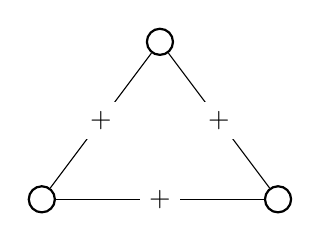
\begin{tikzpicture}
    \tikzstyle{node}=[circle,draw,thick,fill=white]
    \node[node] (A) at (0,0) {};
    \node[node] (B) at (1.5,-2) {};
    \node[node] (C) at (-1.5,-2) {};
    \draw (A) -- (B) node[midway,fill=white]{+};
    \draw (A) -- (C) node[midway,fill=white]{+};
    \draw (B) -- (C) node[midway,fill=white]{+};
    \end{tikzpicture}
    \hspace{2cm}
    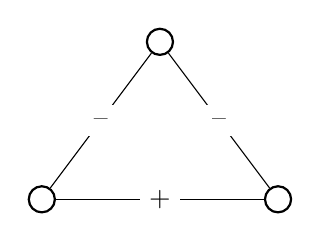
\begin{tikzpicture}
    \tikzstyle{node}=[circle,draw,thick,fill=white]
    \node[node] (A) at (0,0) {};
    \node[node] (B) at (1.5,-2) {};
    \node[node] (C) at (-1.5,-2) {};
    \draw (A) -- (B) node[midway,fill=white]{--};
    \draw (A) -- (C) node[midway,fill=white]{--};
    \draw (B) -- (C) node[midway,fill=white]{+};
    \end{tikzpicture}
    \end{center}

    Exemples de graphes faiblement équilibrés :
    \begin{center}
    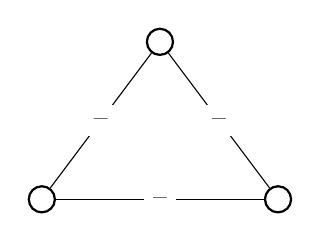
\begin{tikzpicture}
    \tikzstyle{node}=[circle,draw,thick,fill=white]
    \node[node] (A) at (0,0) {};
    \node[node] (B) at (1.5,-2) {};
    \node[node] (C) at (-1.5,-2) {};
    \draw (A) -- (B) node[midway,fill=white]{--};
    \draw (A) -- (C) node[midway,fill=white]{--};
    \draw (B) -- (C) node[midway,fill=white]{--};
    \end{tikzpicture}
    \hspace{2cm}
    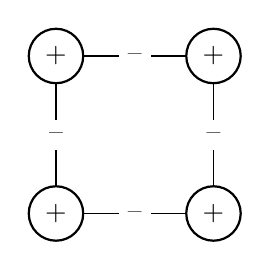
\begin{tikzpicture}
    \tikzstyle{node}=[circle,draw,thick,fill=white]
    \node[node] (A) at (0,0) {+};
    \node[node] (B) at (2,0) {+};
    \node[node] (C) at (2,-2) {+};
    \node[node] (D) at (0,-2) {+};
    \draw (A) -- (B) node[midway,fill=white]{--};
    \draw (A) -- (D) node[midway,fill=white]{--};
    \draw (B) -- (C) node[midway,fill=white]{--};
    \draw (C) -- (D) node[midway,fill=white]{--};
    \end{tikzpicture}
    \end{center}

    Exemple de graphe non équilibré :
    \begin{center}
    \hspace{2cm}
    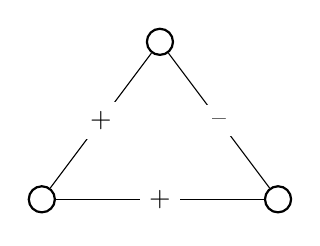
\begin{tikzpicture}
    \tikzstyle{node}=[circle,draw,thick,fill=white]
    \node[node] (A) at (0,0) {};
    \node[node] (B) at (1.5,-2) {};
    \node[node] (C) at (-1.5,-2) {};
    \draw (A) -- (B) node[midway,fill=white]{--};
    \draw (A) -- (C) node[midway,fill=white]{+};
    \draw (B) -- (C) node[midway,fill=white]{+};
    \end{tikzpicture}
    \end{center}

    \noindent \underline{Solution}:

    Le graphe de cette situation peut être représenté comme suit :
    \begin{center}
    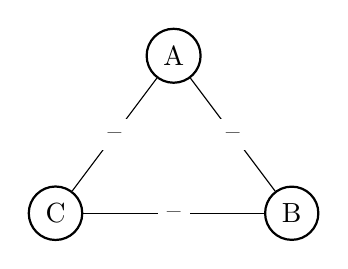
\begin{tikzpicture}
    \tikzstyle{node}=[circle,draw,thick,fill=white]
    \node[node] (A) at (0,0) {A};
    \node[node] (B) at (1.5,-2) {B};
    \node[node] (C) at (-1.5,-2) {C};
    \draw (A) -- (B) node[midway,fill=white]{--};
    \draw (A) -- (C) node[midway,fill=white]{--};
    \draw (B) -- (C) node[midway,fill=white]{--};
    \end{tikzpicture}
    \end{center}

    Avec les noeuds A, B et C tels qu'ils ne contiennent que des $+$.
    On peut donc le retracer :

    \begin{center}
    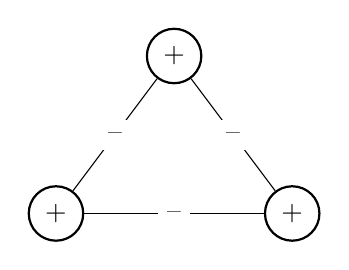
\begin{tikzpicture}
    \tikzstyle{node}=[circle,draw,thick,fill=white]
    \node[node] (A) at (0,0) {+};
    \node[node] (B) at (1.5,-2) {+};
    \node[node] (C) at (-1.5,-2) {+};
    \draw (A) -- (B) node[midway,fill=white]{--};
    \draw (A) -- (C) node[midway,fill=white]{--};
    \draw (B) -- (C) node[midway,fill=white]{--};
    \end{tikzpicture}
    \end{center}

    Ce graphe ne satisfait pas la propriété de balance structurelle.
    En revanche, il respecte l'équilibre faible.\\
    On constate qu'il existe des triangles ($-$, $-$, $-$) : il suffit de prendre 3 personnes issues de 3 villages différents.
    Il n'y a pas de triangles ($+$, $+$, $-$) : pour avoir un lien $-$, il faut prendre 2 personnes de 2 villages différents, et pour avoir un lien $+$ il faut 2 personnes du même village. D'autre part, la présence de tels triangles donnerait un graphe non-équilibré.


\subsection*{Exercice 5}
Soit $K_n$ le graphe complet avec $n \geq 5$ sommets. Supposons que les liens $(1, 2)$, $(2, 3)$, $(3, 4)$, $\ldots$ $(n - 1, n)$, $(n, 1)$ sont positifs et que tous les autres
liens sont n\'{e}gatifs. Pour chaque lien comptez le nombre de triangles balanc\'{e}s et non balanc\'{e}s auxquelles il appartient.

    \subsubsection*{Solution}
    Il y a deux types de triangles balancés :
    \begin{enumerate}
        \item Les triangles composés uniquement de liens positifs : ce graphe n'en compte aucun.
        \item Les triangles composés d'un seul lien positif et de deux liens négatifs : à chaque lien positif correspondent $n-4$ triangles de cette sorte (on retire les 2 noeuds incidents au lien, ainsi que les 2 noeuds qui leur sont adjacents par un lien positif).
    \end{enumerate}

    Il n'y a par contre qu'un seul type de triangle non-balancé contenant un lien positif : les triangles contenant deux liens positifs et un négatif.
    Pour chaque lien positif il y en a $2$ ("un de chaque côté").

    Puisqu'il y a $n$ lien positifs, il y a donc au total $n(n-4)$ triangles balancés. Il y a également $\dfrac{2n}{2}$ triangles non balancés pour ces liens positifs. On divise par deux, car chacun de ces triangles emploie 2 liens positifs.

    On peut vérifier tout cela en comptant le nombre total de triangles possédant un lien positif.
    Ce nombre est $n(n-2) - n = n(n-3)$. Le terme $(n-2)$ vient du fait qu'on compte ici les triangles en prenant les deux noeuds incidents à chaque lien positif. On doit ensuite en retirer $n$, sinon on compterait deux fois chaque triangle composé de deux liens positifs.
    On vérifie donc bien $n(n-4) + n = n(n-3)$, le compte est bon.

\subsection*{Exercice 6}
Si $G$ est complet et non \'{e}quilibr\'{e} est-ce possible d'introduire un nouveau sommet tel que tout les triangles auxquels ce sommet appartient soient \'{e}quilibr\'{e}s?
Si oui donnez une procedure pour le faire. Sinon donnez une preuve.

    \subsubsection*{Solution}
    Si G est complet et non équilibré il est impossible d’introduire un nouveau sommet tel que tous les triangles auxquels ce sommet appartient soient équilibrés en gardant le caractère complet de G.
    En revanche, si l'on ne conserve pas cette propriété, l'opération est possible.\\
    Si G ne possède que des liens négatifs, il suffit de relier un sommet au nouveau par un lien positif, et un autre sommet par un lien négatif.
    On obtiendra ainsi un (et un seul, il est impossible d'en créer plus) triangle ($+$, $-$, $-$), qui est équilibré.\\
    Si G possède des triangles du type ($+$, $+$, $-$), on peut relier le nouveau sommet à deux sommets liés par un lien négatif comme dans le cas précédent ($+$, $-$, $-$) ; ou à deux sommets liés par un lien positif avec deux liens positifs ($+$, $+$, $+$) ; ou à deux sommets liés par un lien positif avec un lien positif et un lien négatif ($+$, $-$, $-$).


\subsection*{Exercice 7}
Soit $G$ un triangle \'{e}quilibr\'{e}. De combien de fa\c{c}ons peut-on ajouter un sommet en gardant l'\'{e}quilibre structurel?

    \subsubsection*{Solution}
    Commençons par le premier type de triangles équilibrés :
    \begin{center}
    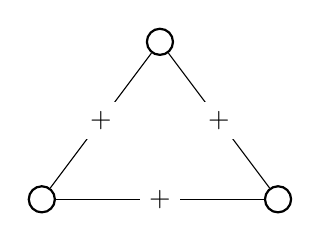
\begin{tikzpicture}
    \tikzstyle{node}=[circle,draw,thick,fill=white]
    \node[node] (A) at (0,0) {};
    \node[node] (B) at (1.5,-2) {};
    \node[node] (C) at (-1.5,-2) {};
    \draw (A) -- (B) node[midway,fill=white]{+};
    \draw (A) -- (C) node[midway,fill=white]{+};
    \draw (B) -- (C) node[midway,fill=white]{+};
    \end{tikzpicture}
    \end{center}

    \begin{center}
    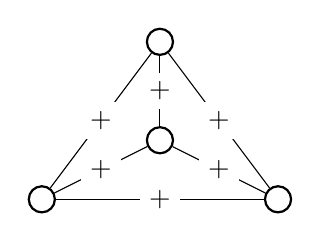
\begin{tikzpicture}
    \tikzstyle{node}=[circle,draw,thick,fill=white]
    \node[node] (A) at (0,0) {};
    \node[node] (B) at (1.5,-2) {};
    \node[node] (C) at (-1.5,-2) {};
    \node[node] (D) at (0,-1.25) {};
    \draw (A) -- (B) node[midway,fill=white]{+};
    \draw (A) -- (C) node[midway,fill=white]{+};
    \draw (B) -- (C) node[midway,fill=white]{+};
    \draw (D) -- (A) node[midway,fill=white]{+};
    \draw (D) -- (B) node[midway,fill=white]{+};
    \draw (D) -- (C) node[midway,fill=white]{+};
    \end{tikzpicture}
    \hspace{0.5cm}
    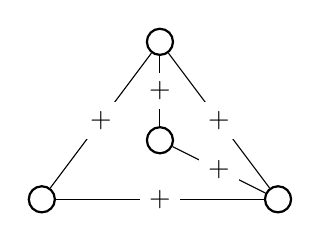
\begin{tikzpicture}
    \tikzstyle{node}=[circle,draw,thick,fill=white]
    \node[node] (A) at (0,0) {};
    \node[node] (B) at (1.5,-2) {};
    \node[node] (C) at (-1.5,-2) {};
    \node[node] (D) at (0,-1.25) {};
    \draw (A) -- (B) node[midway,fill=white]{+};
    \draw (A) -- (C) node[midway,fill=white]{+};
    \draw (B) -- (C) node[midway,fill=white]{+};
    \draw (D) -- (A) node[midway,fill=white]{+};
    \draw (D) -- (B) node[midway,fill=white]{+};
    \end{tikzpicture}
    \hspace{0.5cm}
    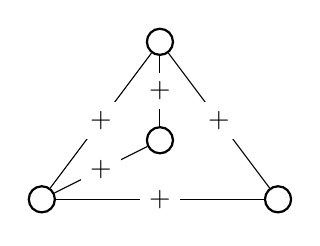
\begin{tikzpicture}
    \tikzstyle{node}=[circle,draw,thick,fill=white]
    \node[node] (A) at (0,0) {};
    \node[node] (B) at (1.5,-2) {};
    \node[node] (C) at (-1.5,-2) {};
    \node[node] (D) at (0,-1.25) {};
    \draw (A) -- (B) node[midway,fill=white]{+};
    \draw (A) -- (C) node[midway,fill=white]{+};
    \draw (B) -- (C) node[midway,fill=white]{+};
    \draw (D) -- (A) node[midway,fill=white]{+};
    \draw (D) -- (C) node[midway,fill=white]{+};
    \end{tikzpicture}
    \hspace{0.5cm}
    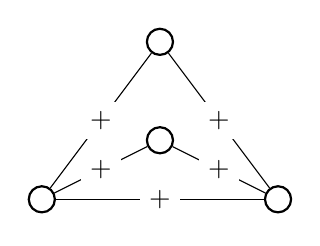
\begin{tikzpicture}
    \tikzstyle{node}=[circle,draw,thick,fill=white]
    \node[node] (A) at (0,0) {};
    \node[node] (B) at (1.5,-2) {};
    \node[node] (C) at (-1.5,-2) {};
    \node[node] (D) at (0,-1.25) {};
    \draw (A) -- (B) node[midway,fill=white]{+};
    \draw (A) -- (C) node[midway,fill=white]{+};
    \draw (B) -- (C) node[midway,fill=white]{+};
    \draw (D) -- (B) node[midway,fill=white]{+};
    \draw (D) -- (C) node[midway,fill=white]{+};
    \end{tikzpicture}

    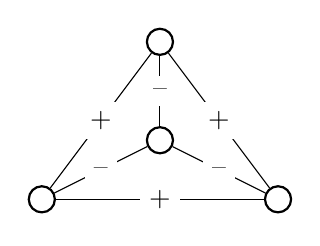
\begin{tikzpicture}
    \tikzstyle{node}=[circle,draw,thick,fill=white]
    \node[node] (A) at (0,0) {};
    \node[node] (B) at (1.5,-2) {};
    \node[node] (C) at (-1.5,-2) {};
    \node[node] (D) at (0,-1.25) {};
    \draw (A) -- (B) node[midway,fill=white]{+};
    \draw (A) -- (C) node[midway,fill=white]{+};
    \draw (B) -- (C) node[midway,fill=white]{+};
    \draw (D) -- (A) node[midway,fill=white]{--};
    \draw (D) -- (B) node[midway,fill=white]{--};
    \draw (D) -- (C) node[midway,fill=white]{--};
    \end{tikzpicture}
    \hspace{0.5cm}
    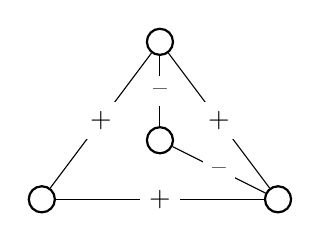
\begin{tikzpicture}
    \tikzstyle{node}=[circle,draw,thick,fill=white]
    \node[node] (A) at (0,0) {};
    \node[node] (B) at (1.5,-2) {};
    \node[node] (C) at (-1.5,-2) {};
    \node[node] (D) at (0,-1.25) {};
    \draw (A) -- (B) node[midway,fill=white]{+};
    \draw (A) -- (C) node[midway,fill=white]{+};
    \draw (B) -- (C) node[midway,fill=white]{+};
    \draw (D) -- (A) node[midway,fill=white]{--};
    \draw (D) -- (B) node[midway,fill=white]{--};
    \end{tikzpicture}
    \hspace{0.5cm}
    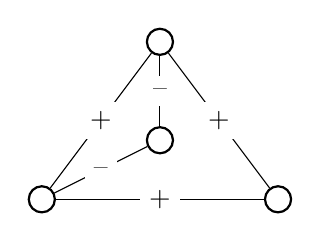
\begin{tikzpicture}
    \tikzstyle{node}=[circle,draw,thick,fill=white]
    \node[node] (A) at (0,0) {};
    \node[node] (B) at (1.5,-2) {};
    \node[node] (C) at (-1.5,-2) {};
    \node[node] (D) at (0,-1.25) {};
    \draw (A) -- (B) node[midway,fill=white]{+};
    \draw (A) -- (C) node[midway,fill=white]{+};
    \draw (B) -- (C) node[midway,fill=white]{+};
    \draw (D) -- (A) node[midway,fill=white]{--};
    \draw (D) -- (C) node[midway,fill=white]{--};
    \end{tikzpicture}
    \hspace{0.5cm}
    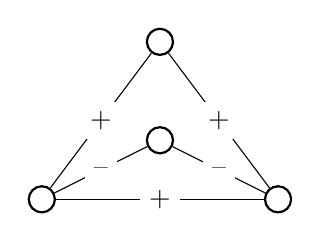
\begin{tikzpicture}
    \tikzstyle{node}=[circle,draw,thick,fill=white]
    \node[node] (A) at (0,0) {};
    \node[node] (B) at (1.5,-2) {};
    \node[node] (C) at (-1.5,-2) {};
    \node[node] (D) at (0,-1.25) {};
    \draw (A) -- (B) node[midway,fill=white]{+};
    \draw (A) -- (C) node[midway,fill=white]{+};
    \draw (B) -- (C) node[midway,fill=white]{+};
    \draw (D) -- (B) node[midway,fill=white]{--};
    \draw (D) -- (C) node[midway,fill=white]{--};
    \end{tikzpicture}
    \end{center}

    Pour le second type de triangles équilibrés :
    \begin{center}
    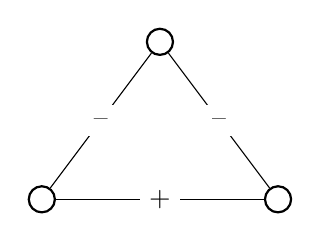
\begin{tikzpicture}
    \tikzstyle{node}=[circle,draw,thick,fill=white]
    \node[node] (A) at (0,0) {};
    \node[node] (B) at (1.5,-2) {};
    \node[node] (C) at (-1.5,-2) {};
    \draw (A) -- (B) node[midway,fill=white]{--};
    \draw (A) -- (C) node[midway,fill=white]{--};
    \draw (B) -- (C) node[midway,fill=white]{+};
    \end{tikzpicture}

    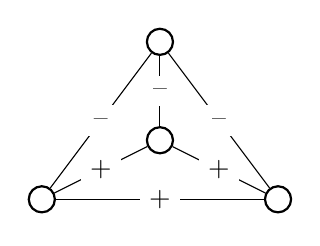
\begin{tikzpicture}
    \tikzstyle{node}=[circle,draw,thick,fill=white]
    \node[node] (A) at (0,0) {};
    \node[node] (B) at (1.5,-2) {};
    \node[node] (C) at (-1.5,-2) {};
    \node[node] (D) at (0,-1.25) {};
    \draw (A) -- (B) node[midway,fill=white]{--};
    \draw (A) -- (C) node[midway,fill=white]{--};
    \draw (B) -- (C) node[midway,fill=white]{+};
    \draw (D) -- (A) node[midway,fill=white]{--};
    \draw (D) -- (B) node[midway,fill=white]{+};
    \draw (D) -- (C) node[midway,fill=white]{+};
    \end{tikzpicture}
    \hspace{0.5cm}
    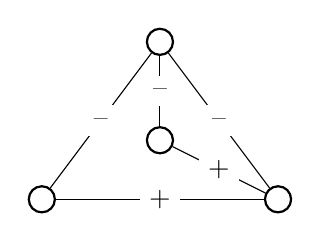
\begin{tikzpicture}
    \tikzstyle{node}=[circle,draw,thick,fill=white]
    \node[node] (A) at (0,0) {};
    \node[node] (B) at (1.5,-2) {};
    \node[node] (C) at (-1.5,-2) {};
    \node[node] (D) at (0,-1.25) {};
    \draw (A) -- (B) node[midway,fill=white]{--};
    \draw (A) -- (C) node[midway,fill=white]{--};
    \draw (B) -- (C) node[midway,fill=white]{+};
    \draw (D) -- (A) node[midway,fill=white]{--};
    \draw (D) -- (B) node[midway,fill=white]{+};
    \end{tikzpicture}
    \hspace{0.5cm}
    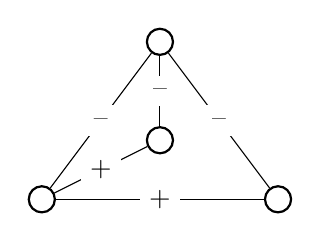
\begin{tikzpicture}
    \tikzstyle{node}=[circle,draw,thick,fill=white]
    \node[node] (A) at (0,0) {};
    \node[node] (B) at (1.5,-2) {};
    \node[node] (C) at (-1.5,-2) {};
    \node[node] (D) at (0,-1.25) {};
    \draw (A) -- (B) node[midway,fill=white]{--};
    \draw (A) -- (C) node[midway,fill=white]{--};
    \draw (B) -- (C) node[midway,fill=white]{+};
    \draw (D) -- (A) node[midway,fill=white]{--};
    \draw (D) -- (C) node[midway,fill=white]{+};
    \end{tikzpicture}
    \hspace{0.5cm}
    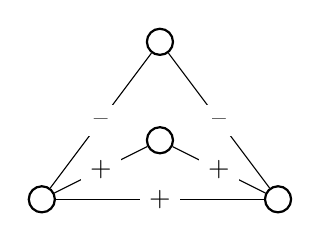
\begin{tikzpicture}
    \tikzstyle{node}=[circle,draw,thick,fill=white]
    \node[node] (A) at (0,0) {};
    \node[node] (B) at (1.5,-2) {};
    \node[node] (C) at (-1.5,-2) {};
    \node[node] (D) at (0,-1.25) {};
    \draw (A) -- (B) node[midway,fill=white]{--};
    \draw (A) -- (C) node[midway,fill=white]{--};
    \draw (B) -- (C) node[midway,fill=white]{+};
    \draw (D) -- (B) node[midway,fill=white]{+};
    \draw (D) -- (C) node[midway,fill=white]{+};
    \end{tikzpicture}

    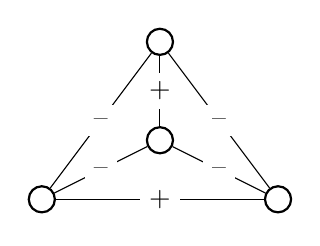
\begin{tikzpicture}
    \tikzstyle{node}=[circle,draw,thick,fill=white]
    \node[node] (A) at (0,0) {};
    \node[node] (B) at (1.5,-2) {};
    \node[node] (C) at (-1.5,-2) {};
    \node[node] (D) at (0,-1.25) {};
    \draw (A) -- (B) node[midway,fill=white]{--};
    \draw (A) -- (C) node[midway,fill=white]{--};
    \draw (B) -- (C) node[midway,fill=white]{+};
    \draw (D) -- (A) node[midway,fill=white]{+};
    \draw (D) -- (B) node[midway,fill=white]{--};
    \draw (D) -- (C) node[midway,fill=white]{--};
    \end{tikzpicture}
    \hspace{0.5cm}
    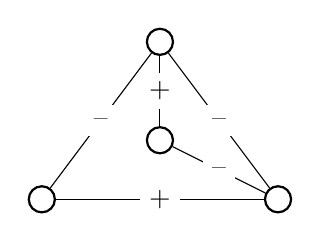
\begin{tikzpicture}
    \tikzstyle{node}=[circle,draw,thick,fill=white]
    \node[node] (A) at (0,0) {};
    \node[node] (B) at (1.5,-2) {};
    \node[node] (C) at (-1.5,-2) {};
    \node[node] (D) at (0,-1.25) {};
    \draw (A) -- (B) node[midway,fill=white]{--};
    \draw (A) -- (C) node[midway,fill=white]{--};
    \draw (B) -- (C) node[midway,fill=white]{+};
    \draw (D) -- (A) node[midway,fill=white]{+};
    \draw (D) -- (B) node[midway,fill=white]{--};
    \end{tikzpicture}
    \hspace{0.5cm}
    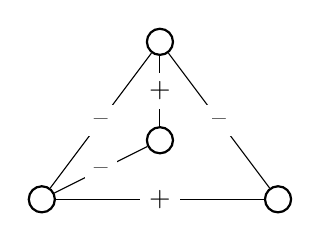
\begin{tikzpicture}
    \tikzstyle{node}=[circle,draw,thick,fill=white]
    \node[node] (A) at (0,0) {};
    \node[node] (B) at (1.5,-2) {};
    \node[node] (C) at (-1.5,-2) {};
    \node[node] (D) at (0,-1.25) {};
    \draw (A) -- (B) node[midway,fill=white]{--};
    \draw (A) -- (C) node[midway,fill=white]{--};
    \draw (B) -- (C) node[midway,fill=white]{+};
    \draw (D) -- (A) node[midway,fill=white]{+};
    \draw (D) -- (C) node[midway,fill=white]{--};
    \end{tikzpicture}
    \hspace{0.5cm}
    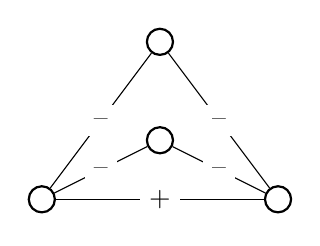
\begin{tikzpicture}
    \tikzstyle{node}=[circle,draw,thick,fill=white]
    \node[node] (A) at (0,0) {};
    \node[node] (B) at (1.5,-2) {};
    \node[node] (C) at (-1.5,-2) {};
    \node[node] (D) at (0,-1.25) {};
    \draw (A) -- (B) node[midway,fill=white]{--};
    \draw (A) -- (C) node[midway,fill=white]{--};
    \draw (B) -- (C) node[midway,fill=white]{+};
    \draw (D) -- (B) node[midway,fill=white]{--};
    \draw (D) -- (C) node[midway,fill=white]{--};
    \end{tikzpicture}
    \end{center}


\subsection*{Exercice 8}
Est-ce que les graphes suivants ont la propri\'{e}t\'{e} d'\'{e}quilibre structurel? Et d'\'{e}quilibre stucturel faible?
\begin{center}
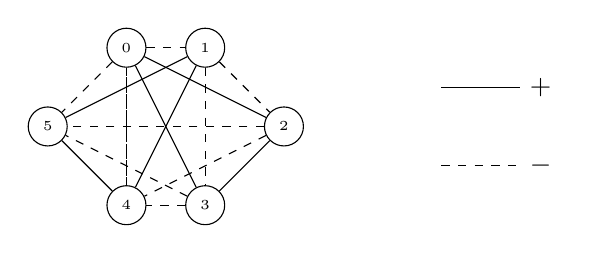
\begin{tikzpicture}
\node[draw, circle] at (0, 0) (a) {\tiny $0$};
\node[draw, circle] at (1, 0) (b) {\tiny $1$};
\node[draw, circle] at (2, -1) (c) {\tiny $2$};
\node[draw, circle] at (1, -2) (d) {\tiny $3$};
\node[draw, circle] at (0, -2) (e) {\tiny $4$};
\node[draw, circle] at (-1, -1) (f) {\tiny $5$};
%\draw (a) -- (0.5, -1) node[anchor=east] {\tiny $+$} -- (d);
%\draw (c) -- (1.5, -1.5) node[anchor=east] {\tiny $+$} -- (d);
%\draw (f) -- (0, -0.5) node {\tiny $+$} -- (b);
%\draw (b) -- (0.5, -1) node {\tiny $+$} -- (e);
\draw (a) -- (d) -- (c) -- (a);
\draw (f) -- (b) -- (e) -- (f);
\draw[dashed] (a) -- (b);
\draw[dashed] (a) -- (e);
\draw[dashed] (a) -- (f);
\draw[dashed] (b) -- (c);
\draw[dashed] (b) -- (d);
\draw[dashed] (c) -- (e);
\draw[dashed] (c) -- (f);
\draw[dashed] (d) -- (e);
\draw[dashed] (d) -- (f);
\draw[dashed] (e) -- (a);

\draw (4, -0.5) -- (5, -0.5) node[anchor = west] {$+$};
\draw[dashed] (4, -1.5) -- (5, -1.5) node[anchor = west] {$-$};
\end{tikzpicture}
\end{center}

\begin{center}
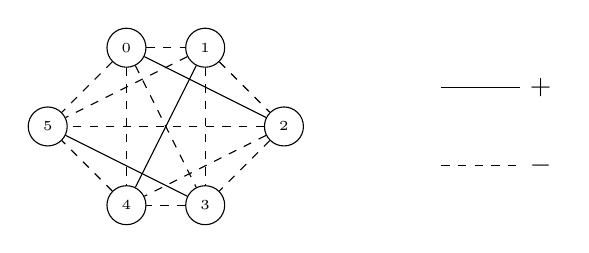
\begin{tikzpicture}
\node[draw, circle] at (0, 0) (a) {\tiny $0$};
\node[draw, circle] at (1, 0) (b) {\tiny $1$};
\node[draw, circle] at (2, -1) (c) {\tiny $2$};
\node[draw, circle] at (1, -2) (d) {\tiny $3$};
\node[draw, circle] at (0, -2) (e) {\tiny $4$};
\node[draw, circle] at (-1, -1) (f) {\tiny $5$};
%\draw (a) -- (0.5, -1) node[anchor=east] {\tiny $+$} -- (d);
%\draw (c) -- (1.5, -1.5) node[anchor=east] {\tiny $+$} -- (d);
%\draw (f) -- (0, -0.5) node {\tiny $+$} -- (b);
%\draw (b) -- (0.5, -1) node {\tiny $+$} -- (e);
\draw[dashed] (a) -- (b);
\draw[] (a) -- (c);
\draw[dashed] (a) -- (d);
\draw[dashed] (a) -- (e);
\draw[dashed] (a) -- (f);
\draw[dashed] (b) -- (c);
\draw[dashed] (b) -- (d);
\draw[] (b) -- (e);
\draw[dashed] (b) -- (f);
\draw[dashed] (c) -- (d);
\draw[dashed] (c) -- (e);
\draw[dashed] (c) -- (f);
\draw[dashed] (d) -- (e);
\draw[] (d) -- (f);
\draw[dashed] (e) -- (f);
\draw (4, -0.5) -- (5, -0.5) node[anchor = west] {$+$};
\draw[dashed] (4, -1.5) -- (5, -1.5) node[anchor = west] {$-$};
\end{tikzpicture}
\end{center}

\begin{center}
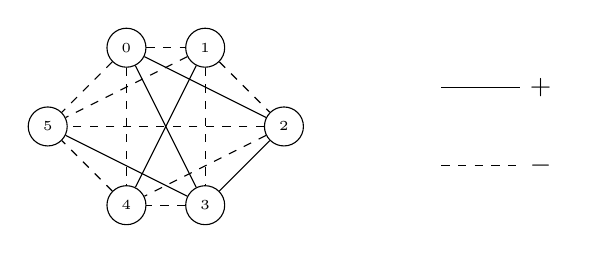
\begin{tikzpicture}
\node[draw, circle] at (0, 0) (a) {\tiny $0$};
\node[draw, circle] at (1, 0) (b) {\tiny $1$};
\node[draw, circle] at (2, -1) (c) {\tiny $2$};
\node[draw, circle] at (1, -2) (d) {\tiny $3$};
\node[draw, circle] at (0, -2) (e) {\tiny $4$};
\node[draw, circle] at (-1, -1) (f) {\tiny $5$};
%\draw (a) -- (0.5, -1) node[anchor=east] {\tiny $+$} -- (d);
%\draw (c) -- (1.5, -1.5) node[anchor=east] {\tiny $+$} -- (d);
%\draw (f) -- (0, -0.5) node {\tiny $+$} -- (b);
%\draw (b) -- (0.5, -1) node {\tiny $+$} -- (e);
\draw[dashed] (a) -- (b);
\draw[] (a) -- (c);
\draw[] (a) -- (d);
\draw[dashed] (a) -- (e);
\draw[dashed] (a) -- (f);
\draw[dashed] (b) -- (c);
\draw[dashed] (b) -- (d);
\draw[] (b) -- (e);
\draw[dashed] (b) -- (f);
\draw[] (c) -- (d);
\draw[dashed] (c) -- (e);
\draw[dashed] (c) -- (f);
\draw[dashed] (d) -- (e);
\draw[] (d) -- (f);
\draw[dashed] (e) -- (f);
\draw (4, -0.5) -- (5, -0.5) node[anchor = west] {$+$};
\draw[dashed] (4, -1.5) -- (5, -1.5) node[anchor = west] {$-$};
\end{tikzpicture}
\end{center}

    \subsubsection*{Solution}
    \begin{itemize}
        \item Ce graphe satisfait la propriété d'équilibre structurel.
        On peut séparer les noeuds en deux groupes : (0, 2, 3) et (1, 4, 5).
        Ces groupes ne contiennent que des liens positifs, et ne sont liés que par des liens négatifs.
        \item Ce graphe ne satisfait pas la propriété d'équilibre.
        Il contient des triangles faiblement équilibrés : (0, 4, 5), (1, 2, 3), (2, 3, 4), ...
        En revanche, il satisfait la propriété d'équilibre faible.
        On peut le séparer en 3 groupes : (0, 2), (1, 4) et (3, 5).
        \item Ce graphe ne satisfait pas la propriété d'équilibre.
        Il contient un triangle non-équilibré : (0, 3, 5).
    \end{itemize}


\subsection*{Exercice 9}
On prends un groupe de $n$ personnes et on ajoute des liens entre chaque paire de personnes avec le signe du lien choisi aléatoirement. Chaque lien est positif avec probabilit\'{e} $\frac{1}{2}$.
Quel est la probabilit\'{e} que le graphe soit structurellement \'{e}quilibr\'{e}?
%Pour quels valeurs de $n$ est-ce que cette probabilit\'{e} est plus grande que $\frac{1}{2}$?

    \subsubsection*{Solution}
    On cherche le rapport du nombre de cas favorables sur le nombre de cas total.\\
    Puisque chaque arête prend 1 valeur parmi 2, et que le graphe est complet, il y a $2^{|E|} = 2^{\frac{n(n-1)}{2}} = 2^{\frac{n^2-n}{2}}$ cas possibles.\\
    On a $\frac{2^n}{2}$ cas favorables. \textbf{TODO : RAISONNEMENT}\\
    On a donc une probabilité de :
    $$ \dfrac{\dfrac{2^n}{2}}{2^{\frac{n^2-n}{2}}} = \dfrac{1}{2^{\frac{n^2-3n+2}{2}}}$$
    \noindent Cette probabilité vaut donc 0.5 dans le cas où $n=3$.
    Ce qui est logique, puisque dans ce cas on a 8 triangles possibles, dont 4 sont équilibrés.



